\chapter{STRique Repeat Detection}
\label{sec:strique}

\begin{figure}[h]
    \centering
    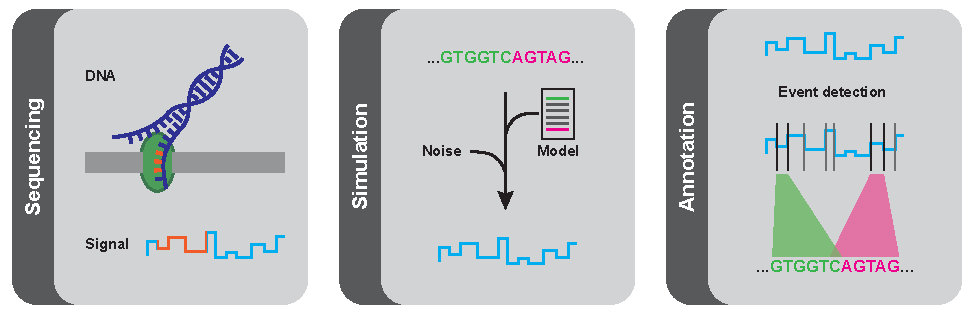
\includegraphics[width=1.0\textwidth]{figures/strique/GA.pdf}
    \label{fig:strique:ga}
\end{figure}


\section{Background}
\label{sec:strique:background}

\section{Data Generation}
\label{sec:strique:data}

\section{Repeat Quantification}
\label{sec:strique:quantification}

\section{Base Modification Detection}
\label{sec:strique:modifications}

\section{Summary}
\label{sec:strique:summary}
